\section{Date: 2026-10-07}
\noindent \textbf{Series ID: EQTA35} 

\noindent This series is titled Total Equity to Total Assets, Banks with Total Assets from \$1B to \$10B, South Atlantic Census Division (DISCONTINUED) and has a frequency of Quarterly, End of Period. The units are Percent and the seasonal adjustment is Not Seasonally Adjusted.The observation start date is 1988-01-01 and the observation end date is 2020-07-01.The popularity of this series is 1. \\ 

\noindent \textbf{Series ID: CCUSSP01IFM650N} 

\noindent This series is titled Currency Conversions: US Dollar Exchange Rate: Spot, End of Period: USD: National Currency for SDR and has a frequency of Monthly. The units are Special Drawing Rights and the seasonal adjustment is Not Seasonally Adjusted.The observation start date is 1975-01-01 and the observation end date is 2023-12-01.The popularity of this series is 13. \\ 

\subsection{Raw Regression}
\noindent Regresses the two series against each other directly. A significant result here can come just as easily from both series sharing a long-run trend as from any real relationship.

\begin{center}
\begin{tabular}{lclc}
\toprule
\textbf{Dep. Variable:}      & value\_fred\_CCUSSP01IFM650N & \textbf{  R-squared:         } &     0.067   \\
\textbf{Model:}              &             OLS              & \textbf{  Adj. R-squared:    } &     0.060   \\
\textbf{Method:}             &        Least Squares         & \textbf{  F-statistic:       } &     9.266   \\
\textbf{Date:}               &       Wed, 07 Oct 2026       & \textbf{  Prob (F-statistic):} &  0.00283    \\
\textbf{Time:}               &           18:02:18           & \textbf{  Log-Likelihood:    } &    133.95   \\
\textbf{No. Observations:}   &               131            & \textbf{  AIC:               } &    -263.9   \\
\textbf{Df Residuals:}       &               129            & \textbf{  BIC:               } &    -258.1   \\
\textbf{Df Model:}           &                 1            & \textbf{                     } &             \\
\textbf{Covariance Type:}    &          nonrobust           & \textbf{                     } &             \\
\bottomrule
\end{tabular}
\begin{tabular}{lcccccc}
                             & \textbf{coef} & \textbf{std err} & \textbf{t} & \textbf{P$> |$t$|$} & \textbf{[0.025} & \textbf{0.975]}  \\
\midrule
\textbf{const}               &       1.2811  &        0.049     &    26.190  &         0.000        &        1.184    &        1.378     \\
\textbf{value\_fred\_EQTA35} &       0.0142  &        0.005     &     3.044  &         0.003        &        0.005    &        0.023     \\
\bottomrule
\end{tabular}
\begin{tabular}{lclc}
\textbf{Omnibus:}       &  3.573 & \textbf{  Durbin-Watson:     } &    0.175  \\
\textbf{Prob(Omnibus):} &  0.168 & \textbf{  Jarque-Bera (JB):  } &    2.476  \\
\textbf{Skew:}          &  0.161 & \textbf{  Prob(JB):          } &    0.290  \\
\textbf{Kurtosis:}      &  2.409 & \textbf{  Cond. No.          } &     67.4  \\
\bottomrule
\end{tabular}
%\caption{OLS Regression Results}
\end{center}

Notes: \newline
 [1] Standard Errors assume that the covariance matrix of the errors is correctly specified.

\begin{figure}
\centering
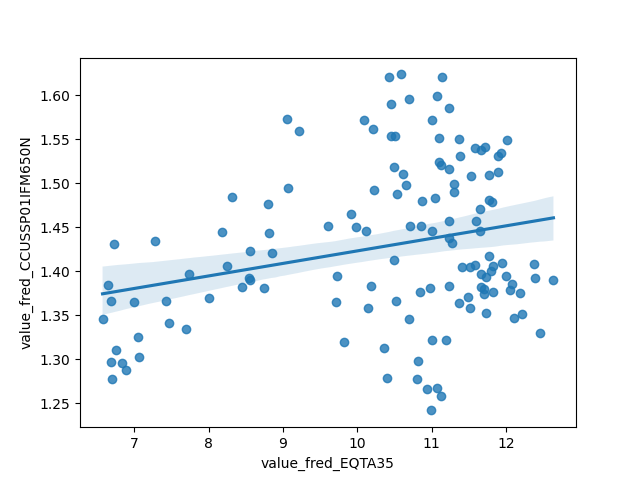
\includegraphics[scale = 0.9]{plots/plot_2026-10-07.png}
\caption{Raw Regression Plot for 2026-10-07}
\end{figure}
\newpage
\subsection{Detrended Regression}
\noindent Regresses the residuals of each series after removing its own linear time trend, so a shared trend can no longer drive the result on its own. A relationship that stays significant here is better evidence of a genuine link between the two series.

\begin{center}
\begin{tabular}{lclc}
\toprule
\textbf{Dep. Variable:}                 & value\_fred\_CCUSSP01IFM650N\_detrended & \textbf{  R-squared:         } &     0.004   \\
\textbf{Model:}                         &                   OLS                   & \textbf{  Adj. R-squared:    } &    -0.003   \\
\textbf{Method:}                        &              Least Squares              & \textbf{  F-statistic:       } &    0.5577   \\
\textbf{Date:}                          &             Wed, 07 Oct 2026            & \textbf{  Prob (F-statistic):} &    0.457    \\
\textbf{Time:}                          &                 18:02:18                & \textbf{  Log-Likelihood:    } &    139.59   \\
\textbf{No. Observations:}              &                     131                 & \textbf{  AIC:               } &    -275.2   \\
\textbf{Df Residuals:}                  &                     129                 & \textbf{  BIC:               } &    -269.4   \\
\textbf{Df Model:}                      &                       1                 & \textbf{                     } &             \\
\textbf{Covariance Type:}               &                nonrobust                & \textbf{                     } &             \\
\bottomrule
\end{tabular}
\begin{tabular}{lcccccc}
                                        & \textbf{coef} & \textbf{std err} & \textbf{t} & \textbf{P$> |$t$|$} & \textbf{[0.025} & \textbf{0.975]}  \\
\midrule
\textbf{const}                          &    3.906e-14  &        0.007     &  5.32e-12  &         1.000        &       -0.015    &        0.015     \\
\textbf{value\_fred\_EQTA35\_detrended} &      -0.0055  &        0.007     &    -0.747  &         0.457        &       -0.020    &        0.009     \\
\bottomrule
\end{tabular}
\begin{tabular}{lclc}
\textbf{Omnibus:}       & 10.155 & \textbf{  Durbin-Watson:     } &    0.184  \\
\textbf{Prob(Omnibus):} &  0.006 & \textbf{  Jarque-Bera (JB):  } &    4.169  \\
\textbf{Skew:}          &  0.123 & \textbf{  Prob(JB):          } &    0.124  \\
\textbf{Kurtosis:}      &  2.162 & \textbf{  Cond. No.          } &     1.00  \\
\bottomrule
\end{tabular}
%\caption{OLS Regression Results}
\end{center}

Notes: \newline
 [1] Standard Errors assume that the covariance matrix of the errors is correctly specified.

\begin{figure}
\centering
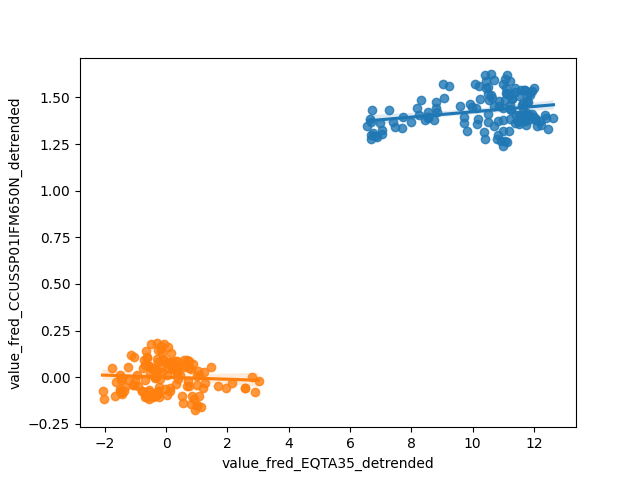
\includegraphics[scale = 0.9]{plots/plot_2026-10-07_detrended.png}
\caption{Detrended Regression Plot for 2026-10-07}
\end{figure}
\newpage
